% -*- Mode:LaTeX -*-

\documentclass[twocolumn,prl,superscriptaddress]{revtex4}

% Required packages
\usepackage{dcolumn}
\usepackage{amsmath}
%\usepackage{calrsfs}

% Optional extra packages
\usepackage{graphicx}
\usepackage{subfigure}

% Can delete this at the end
\usepackage{comment}

% Style parameters
\setlength{\parskip}{0pt}
\setlength{\tabcolsep}{6pt}
\setlength{\arraycolsep}{2pt}

% Macros

\newcommand{\dd}{\mathrm{d}}
\newcommand{\ii}{\mathrm{i}}
\newcommand{\e}{\mathrm{e}}
\newcommand{\half}{\tfrac12}
\newcommand{\set}[1]{\lbrace#1\rbrace}
\newcommand{\av}[1]{\left\langle#1\right\rangle}
\newcommand{\etal}{{\it{}et~al.}}
\newcommand{\defn}{\textit}
\newcommand{\Ord}{\mathrm{O}}
\newcommand{\Tr}{\mathop\mathrm{Tr}}
\newcommand{\erf}{\mathop\mathrm{erf}}
\renewcommand{\Im}{\mathop\mathrm{Im}}
\newcommand{\mat}{\mathbf}
\renewcommand{\vec}{\mathbf}
\newcommand\Beta{\mathrm{B}}
\newcommand\colora{black }
\newcommand\colorb{red }
\newcommand\colorc{green }

\newcommand\pin{p_\textrm{in}}
\newcommand\pout{p_\textrm{out}}
\newcommand\cin{c_\textrm{in}}
\newcommand\cout{c_\textrm{out}}


\begin{document}

\title{An improved eigenvector centrality based on the non-backtracking matrix}
\author{Travis Martin}
\affiliation{Department of Electrical Engineering and Computer Science,
  University of Michigan, Ann Arbor, MI 48109}
\author{Xiao Zhang}
\affiliation{Department of Physics, University of Michigan, Ann Arbor, MI 48109}
\author{M. E. J. Newman}
\affiliation{Department of Physics and Center for the Study of Complex Systems, University of Michigan, Ann Arbor, MI 48109}

\begin{abstract}
  We show that eigenvector centrality behaves poorly on sparse random networks with vertices of unusually high degree, or hubs. We give numerical and analytical evidence that traditional eigenvector centrality is susceptible to localization, giving disproportionately high centrality to hubs and their neighbors. We propose an alternative centrality measure, \emph{non-backtracking centrality}, which converges to eigenvector centrality for dense networks and avoids the problem of localization around hubs in sparse networks.
\end{abstract}

\maketitle

Network researchers have long been interested in an effective method of measuring \emph{centrality}, a quantification of how important or central each network node is. Eigenvector centrality~\cite{bonacich72} is among the most influential centrality measures, with widely ranging applications to metabolic networks~\cite{ding10}, football team ranking~\cite{keener93}, bird mating analysis~\cite{ryder08}, and Google's highly successful PageRank algorithm\footnote{PageRank uses a closely related variant of eigenvector centrality}~\cite{page99}. Eigenvector centrality specifies that each node's centrality be proportional to the sum of its neighbor's centralities, and can be conveniently calculated from the leading eigenvector of the network's adjacency matrix. Chung~\etal\ show that the largest eigenvalue of the adjacency matrix of a random graph model is almost surely determined by the larger of the square root of the maximum degree, $\sqrt{m}$, and the weighted average of the squares of the expected degrees, $\tilde{d}$~\cite{chung03}. In this paper we show that, at least for the Poisson with planted hub and power-law random graph families, eigenvector centrality fails when the leading eigenvalue corresponds to $\sqrt{m}$ by giving a centrality vector which is too-localized around the highest degree node. In the second half of this paper we introduce \emph{non-backtracking centrality}, calculated from an alternative network representation called the non-backtracking matrix~\cite{krzakala13} or Hashimoto edge matrix~\cite{hashimoto89}, which avoids this failure case of eigenvector centrality while remaining asymptotically equal in the dense limit.

We first consider the Poisson random graph with nodes of identical expected degree $c$ and a planted hub of expected degree $k_n$. In Fig.~\ref{fig:transition} we display eigenvector (left column) and non-backtracking (right column) centralities for the hub and all nodes within distance 2, from the same Poisson random graph with size $n=1000000$ and $c = 10$. The rows show increasing hub size, from $k_n = 20$, $k_n = 70$, and $k_n = 120$. The eigenvector centralities, which are proportional to node areas, increase dramatically from $k_n = 70$ to $k_n = 120$ while the non-backtracking centralities increase steadily. We demonstrate below that this sudden increase in centrality is an undesirable side-effect of a phase transition in the leading eigenvalue.

%talk about global vs local??

\begin{figure}
\begin{center}
        \subfigure{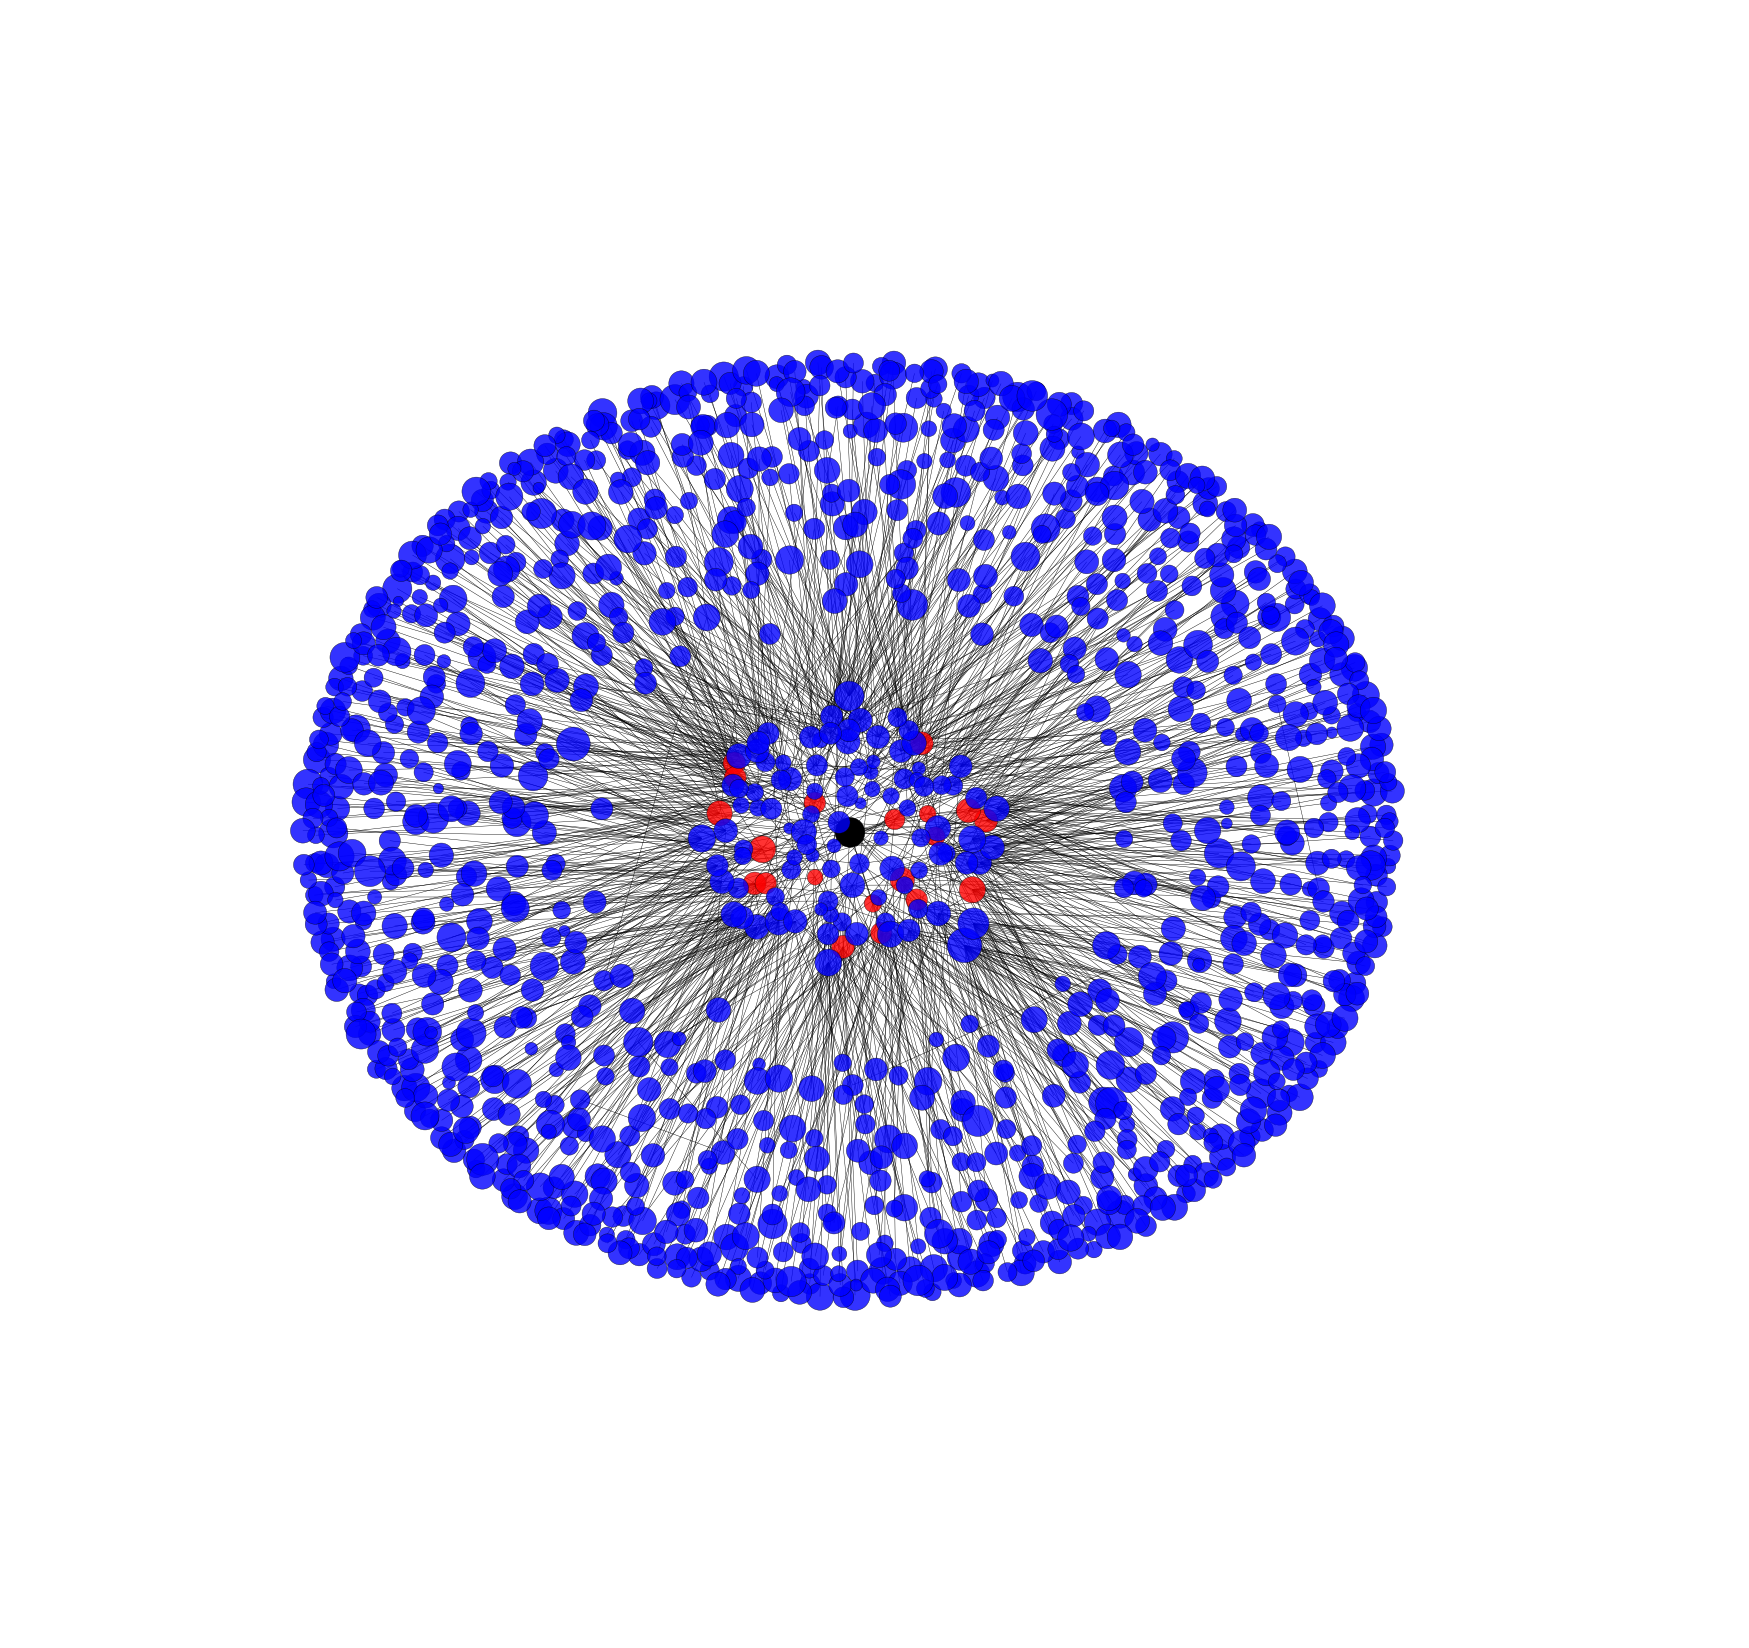
\includegraphics[width=0.49\columnwidth]{1.png}}
        \subfigure{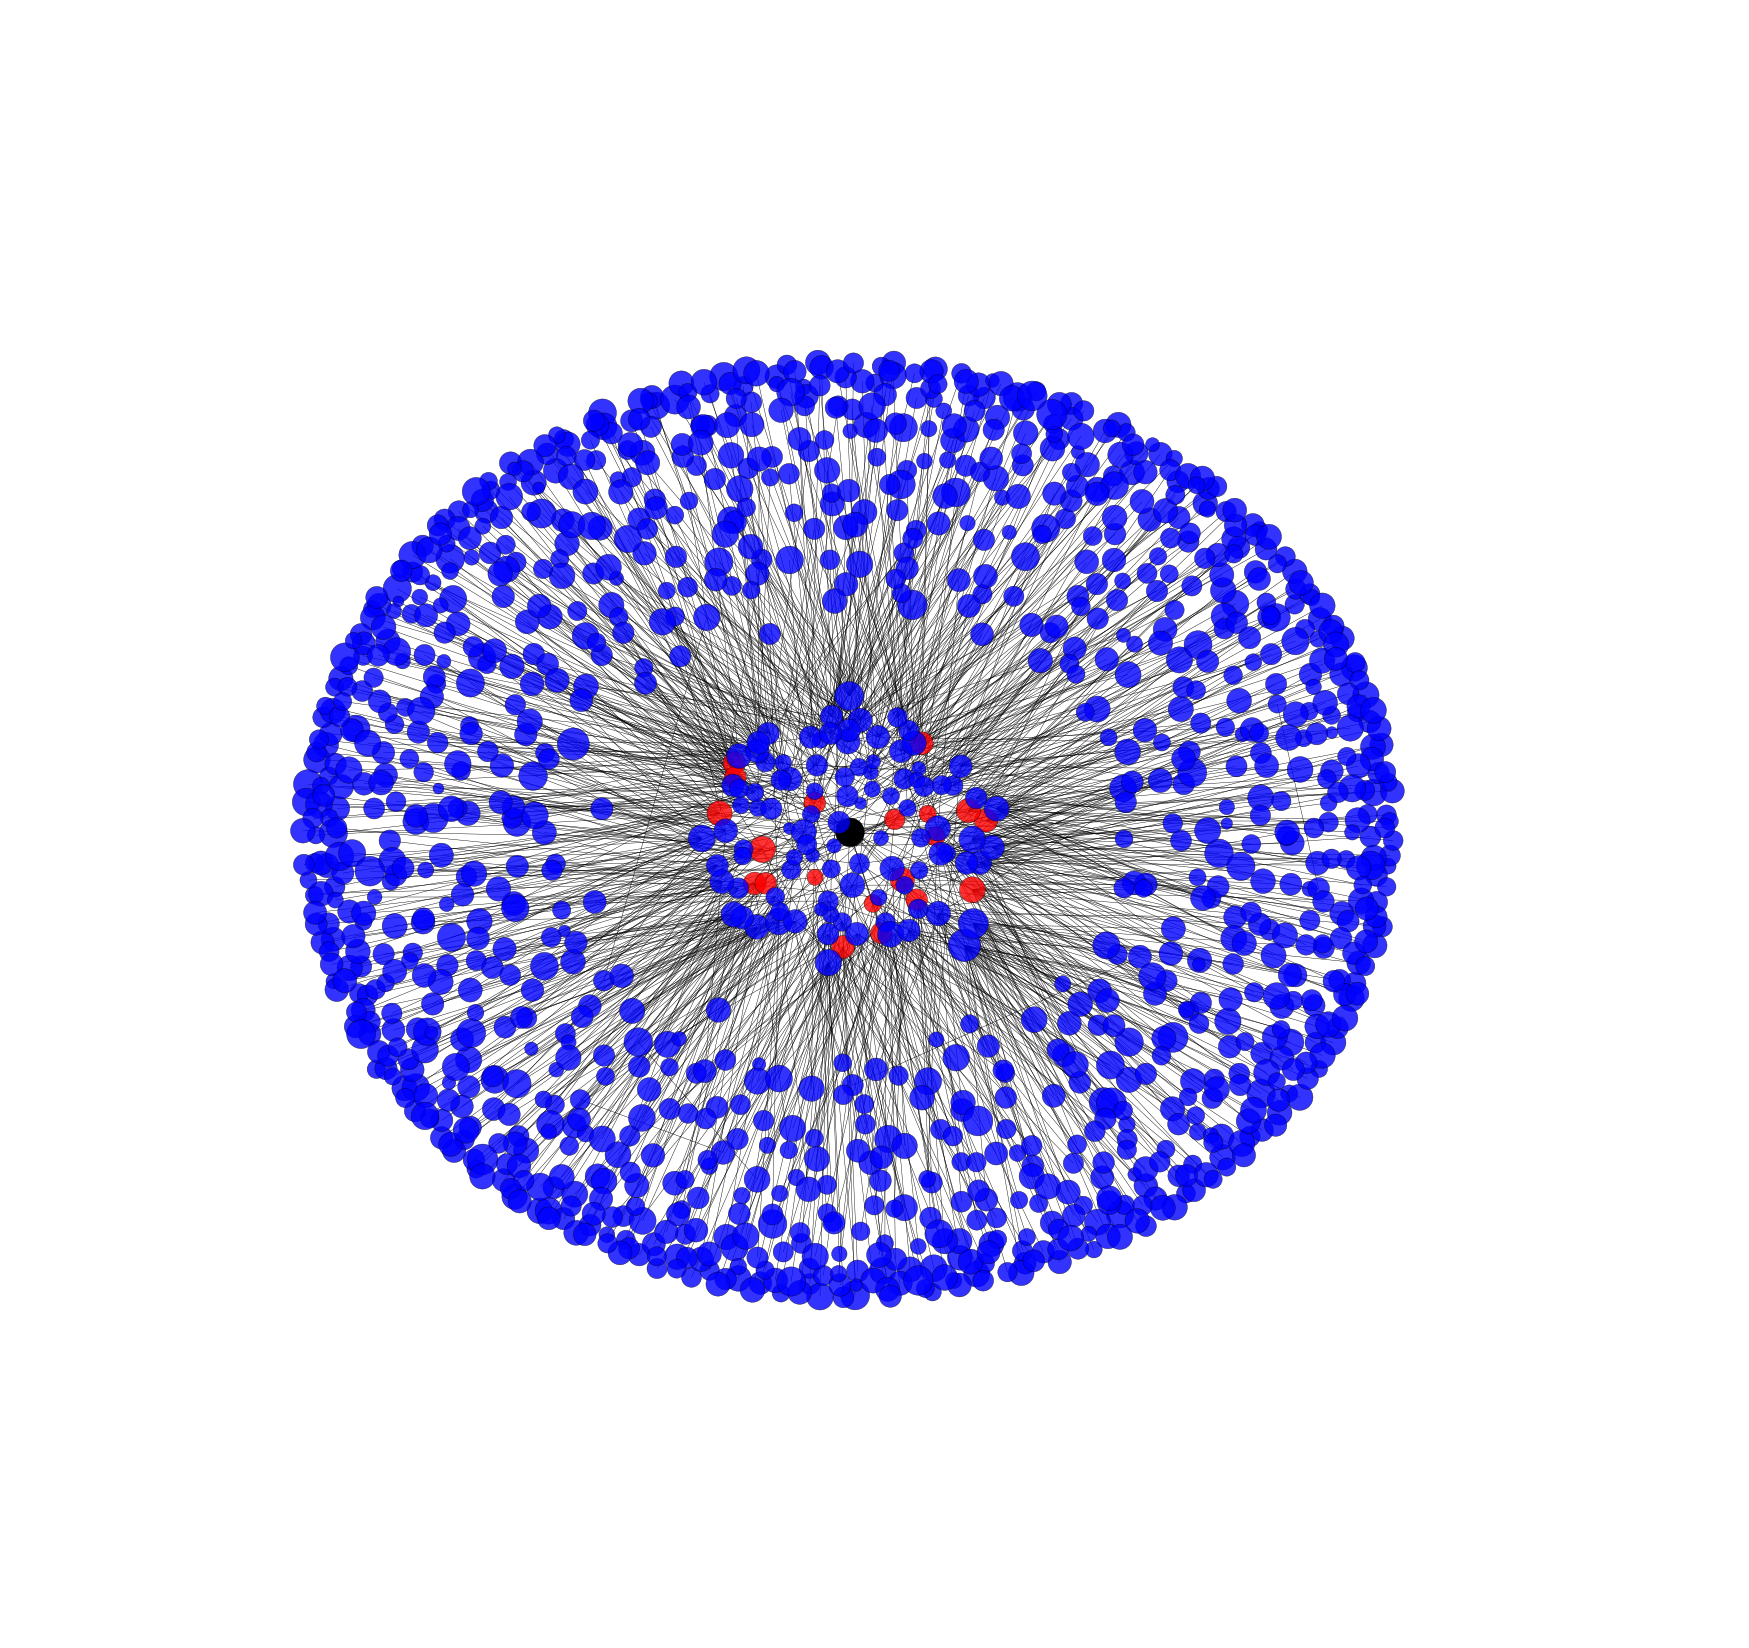
\includegraphics[width=0.49\columnwidth]{1h.png}}
        \subfigure{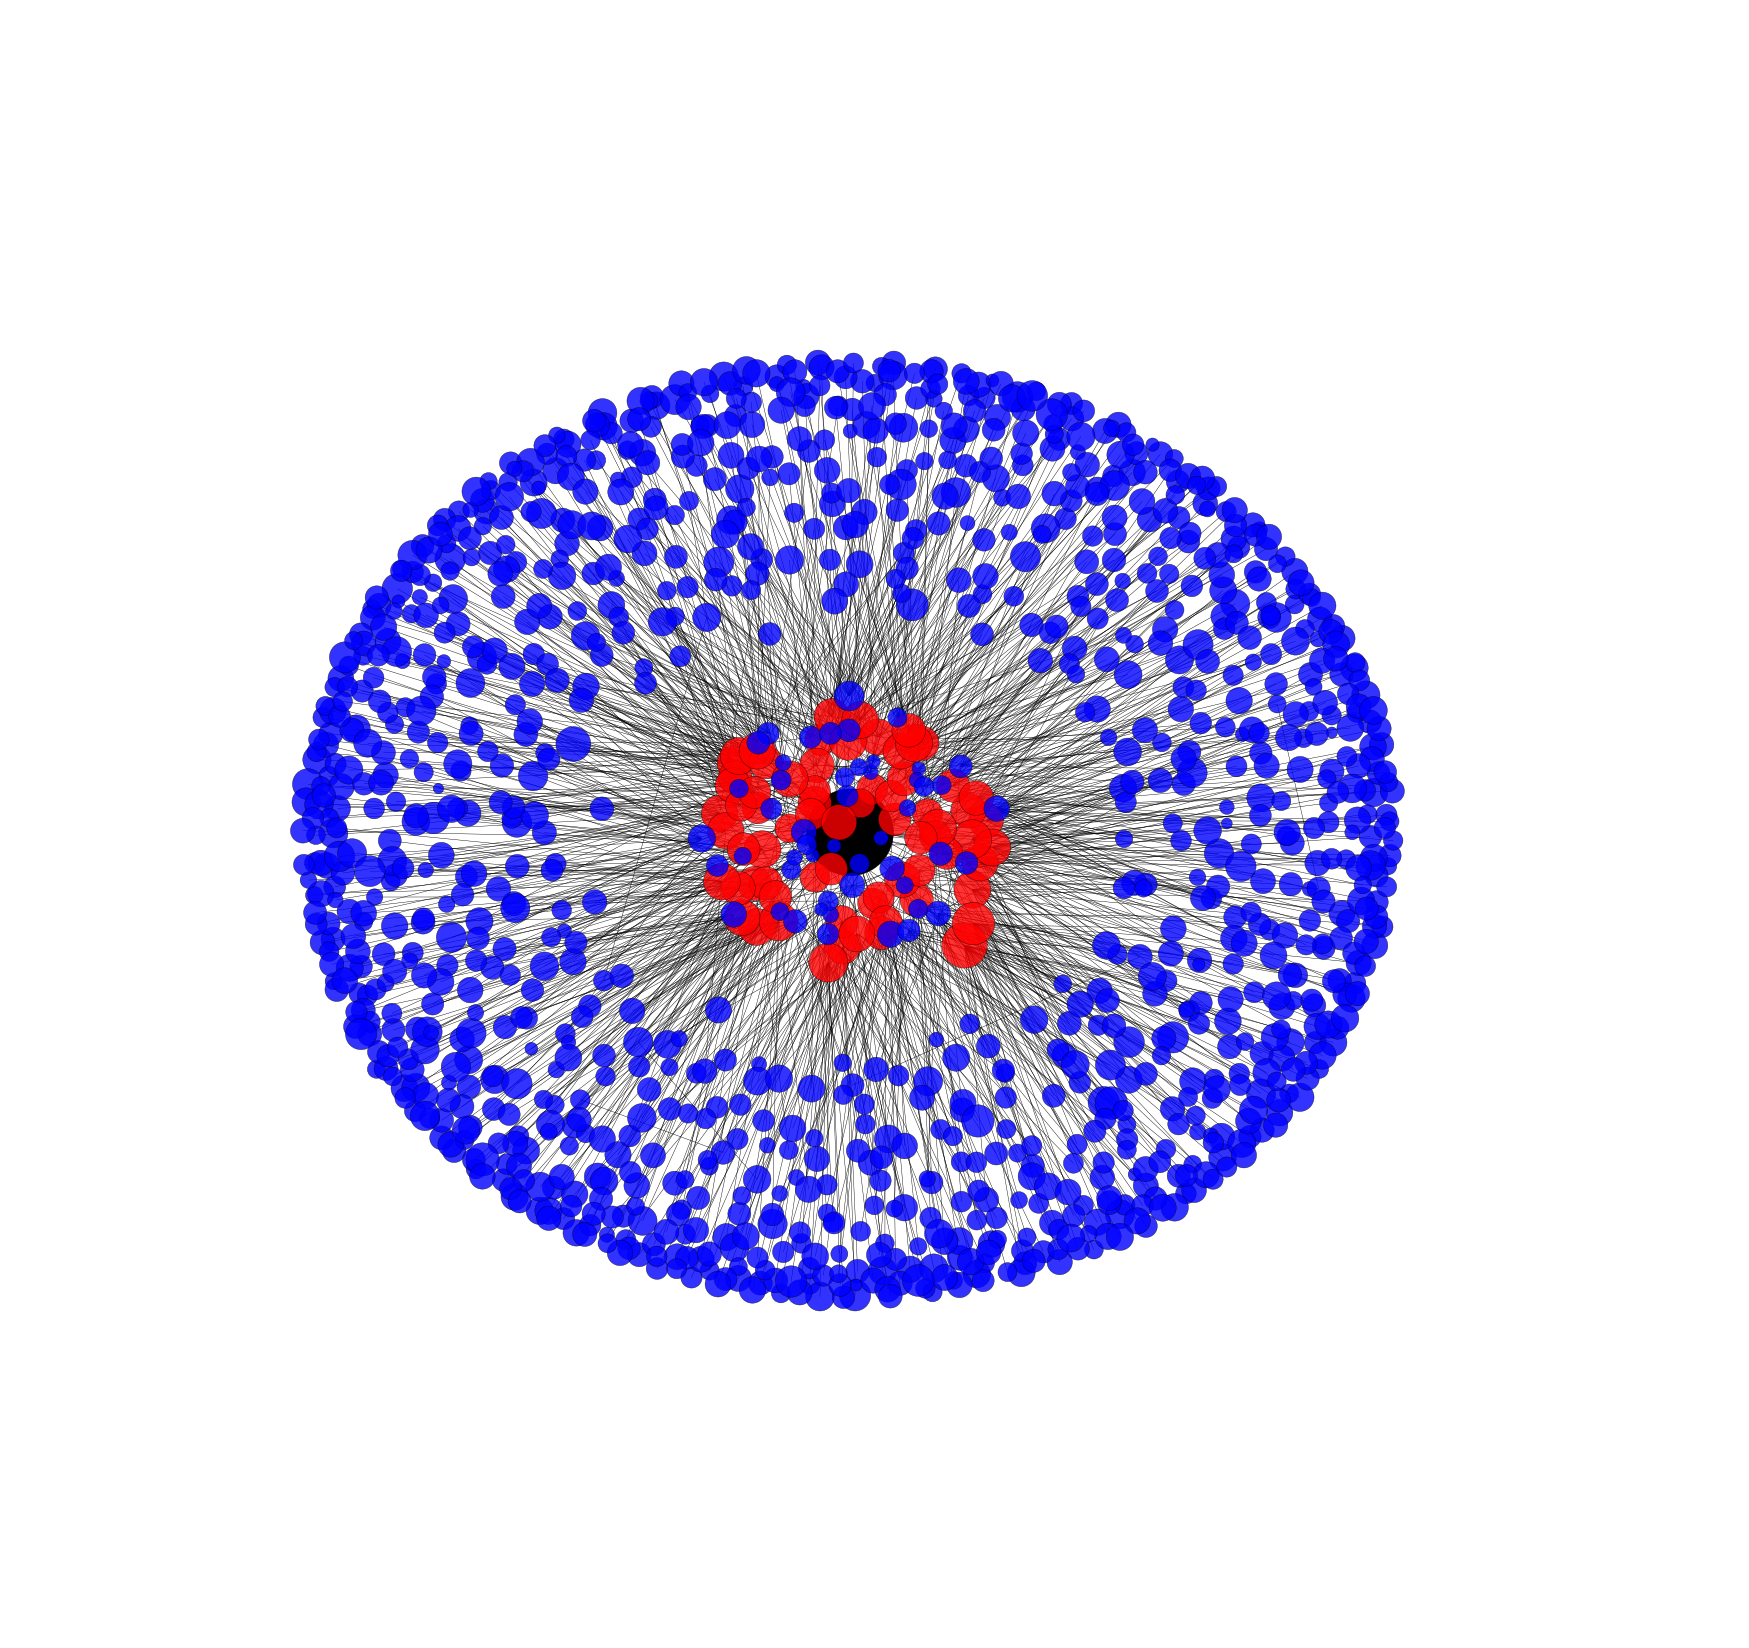
\includegraphics[width=0.49\columnwidth]{2.png}}
        \subfigure{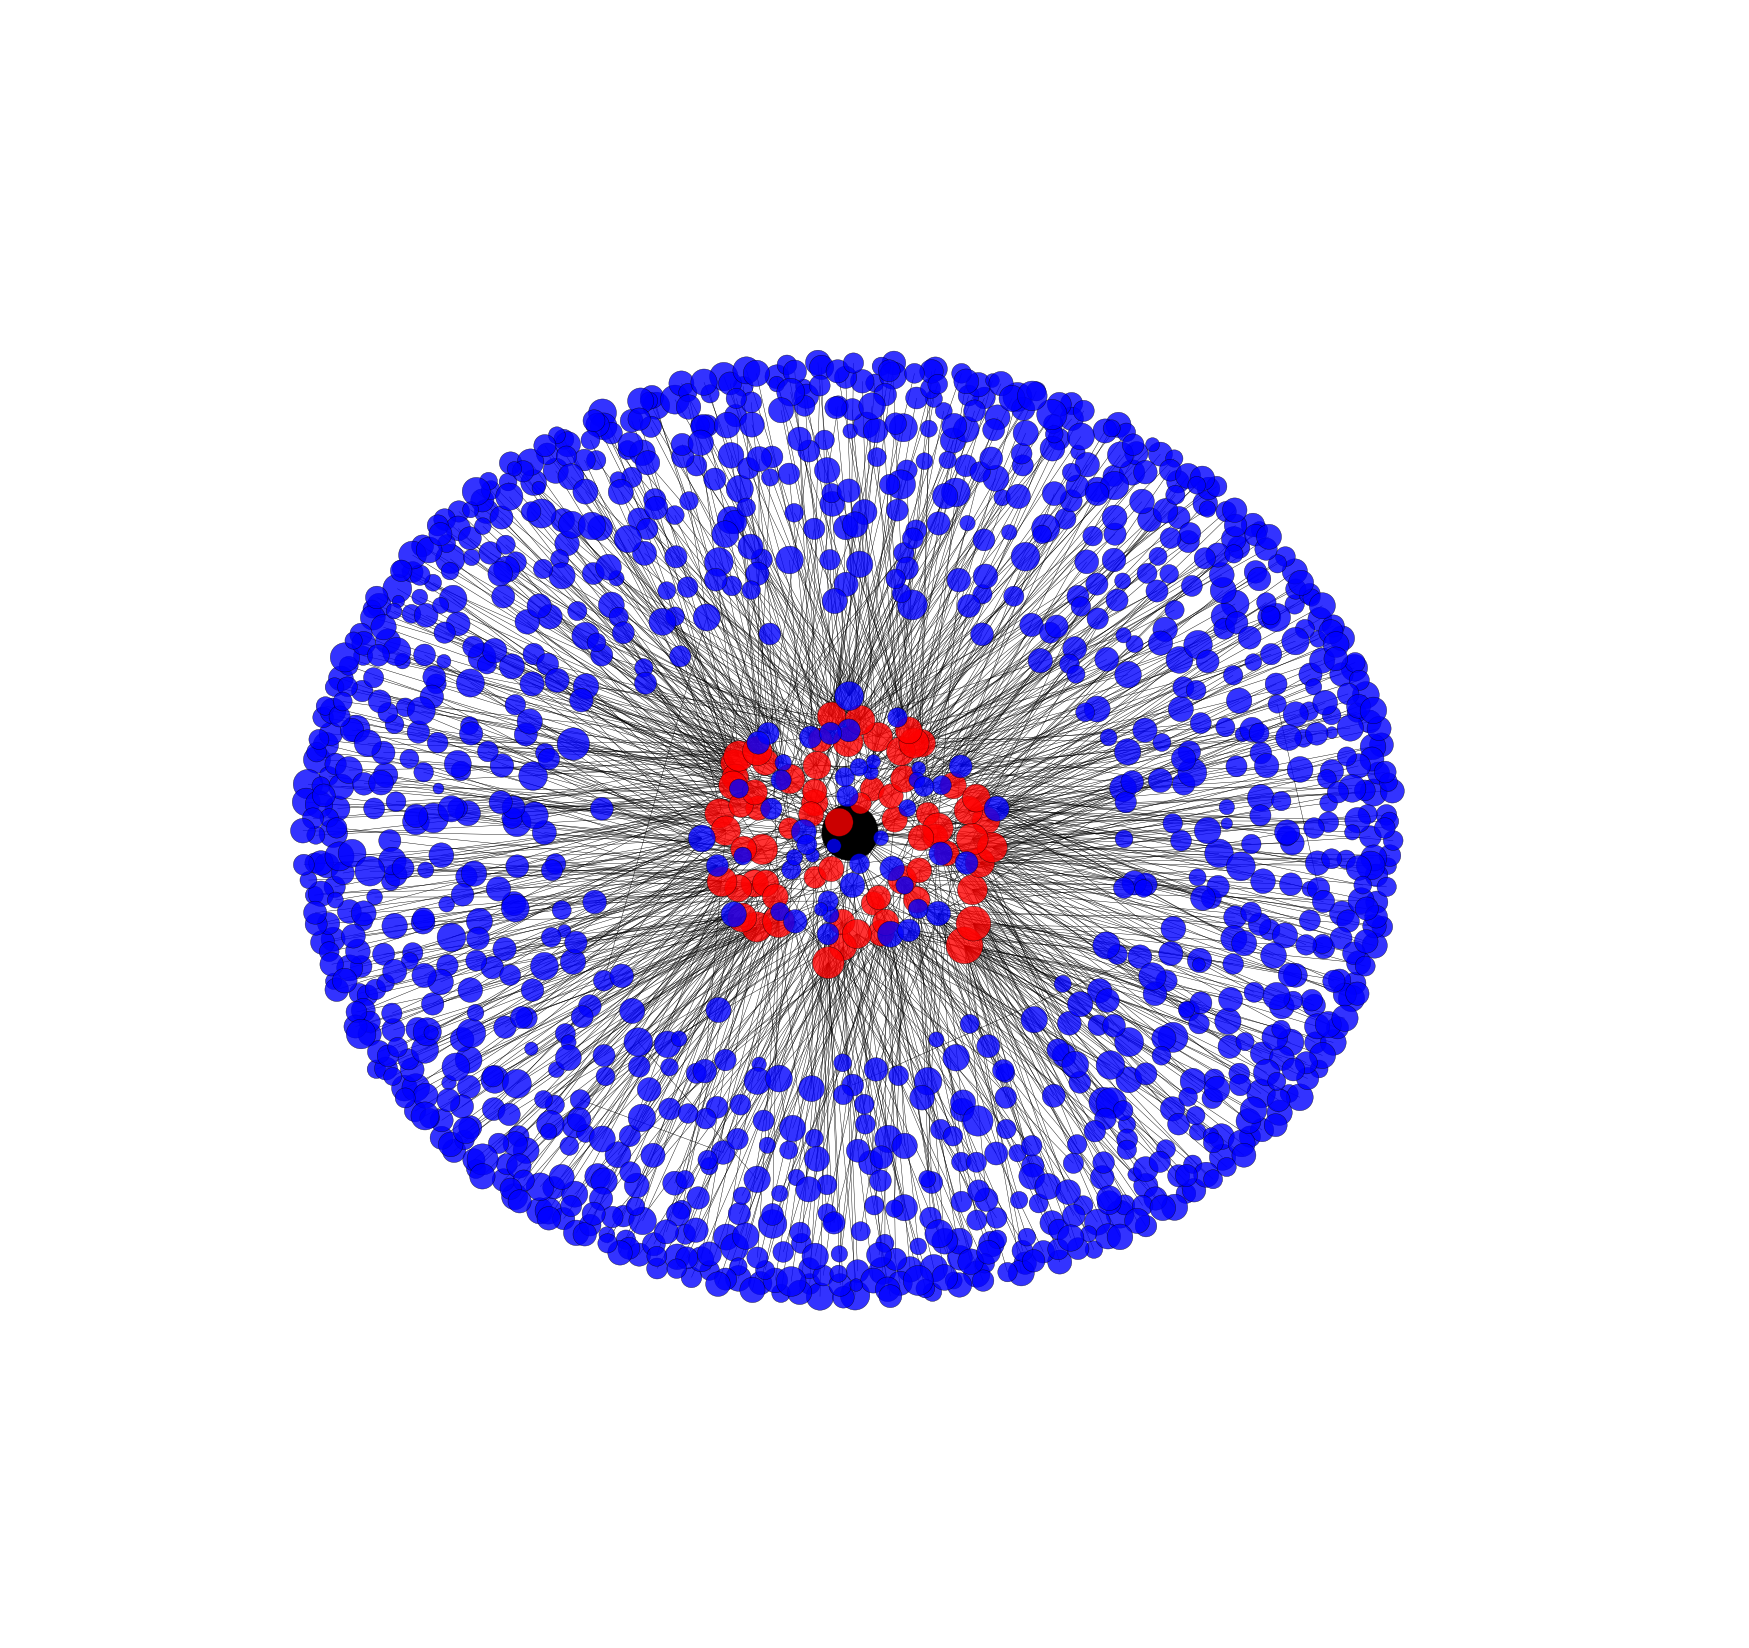
\includegraphics[width=0.49\columnwidth]{2h.png}}
        \subfigure{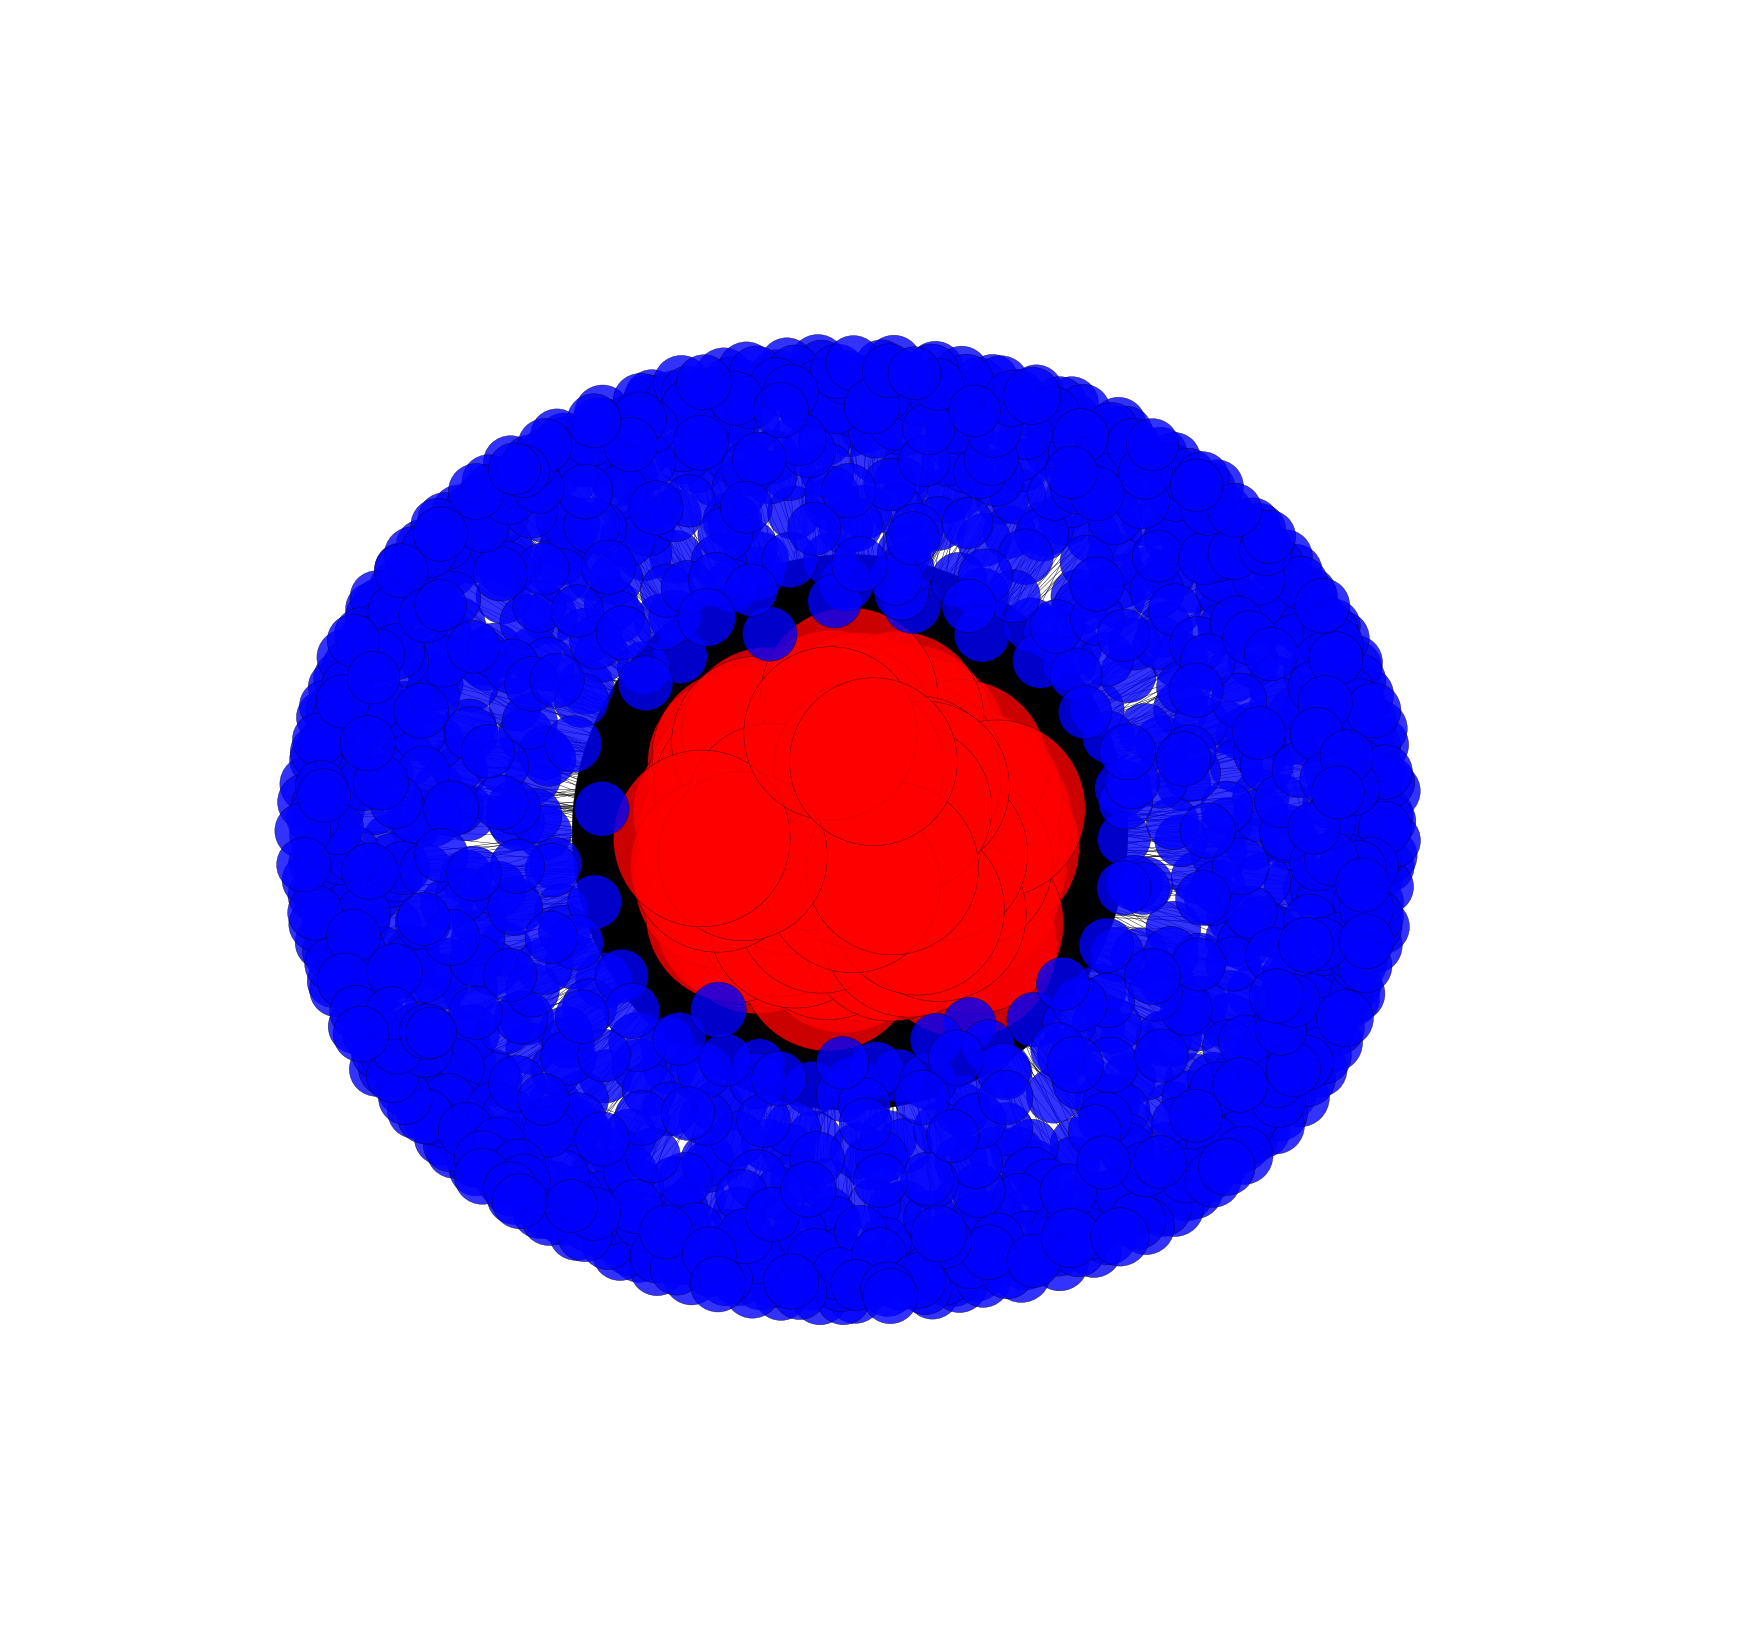
\includegraphics[width=0.49\columnwidth]{3.png}}
        \subfigure{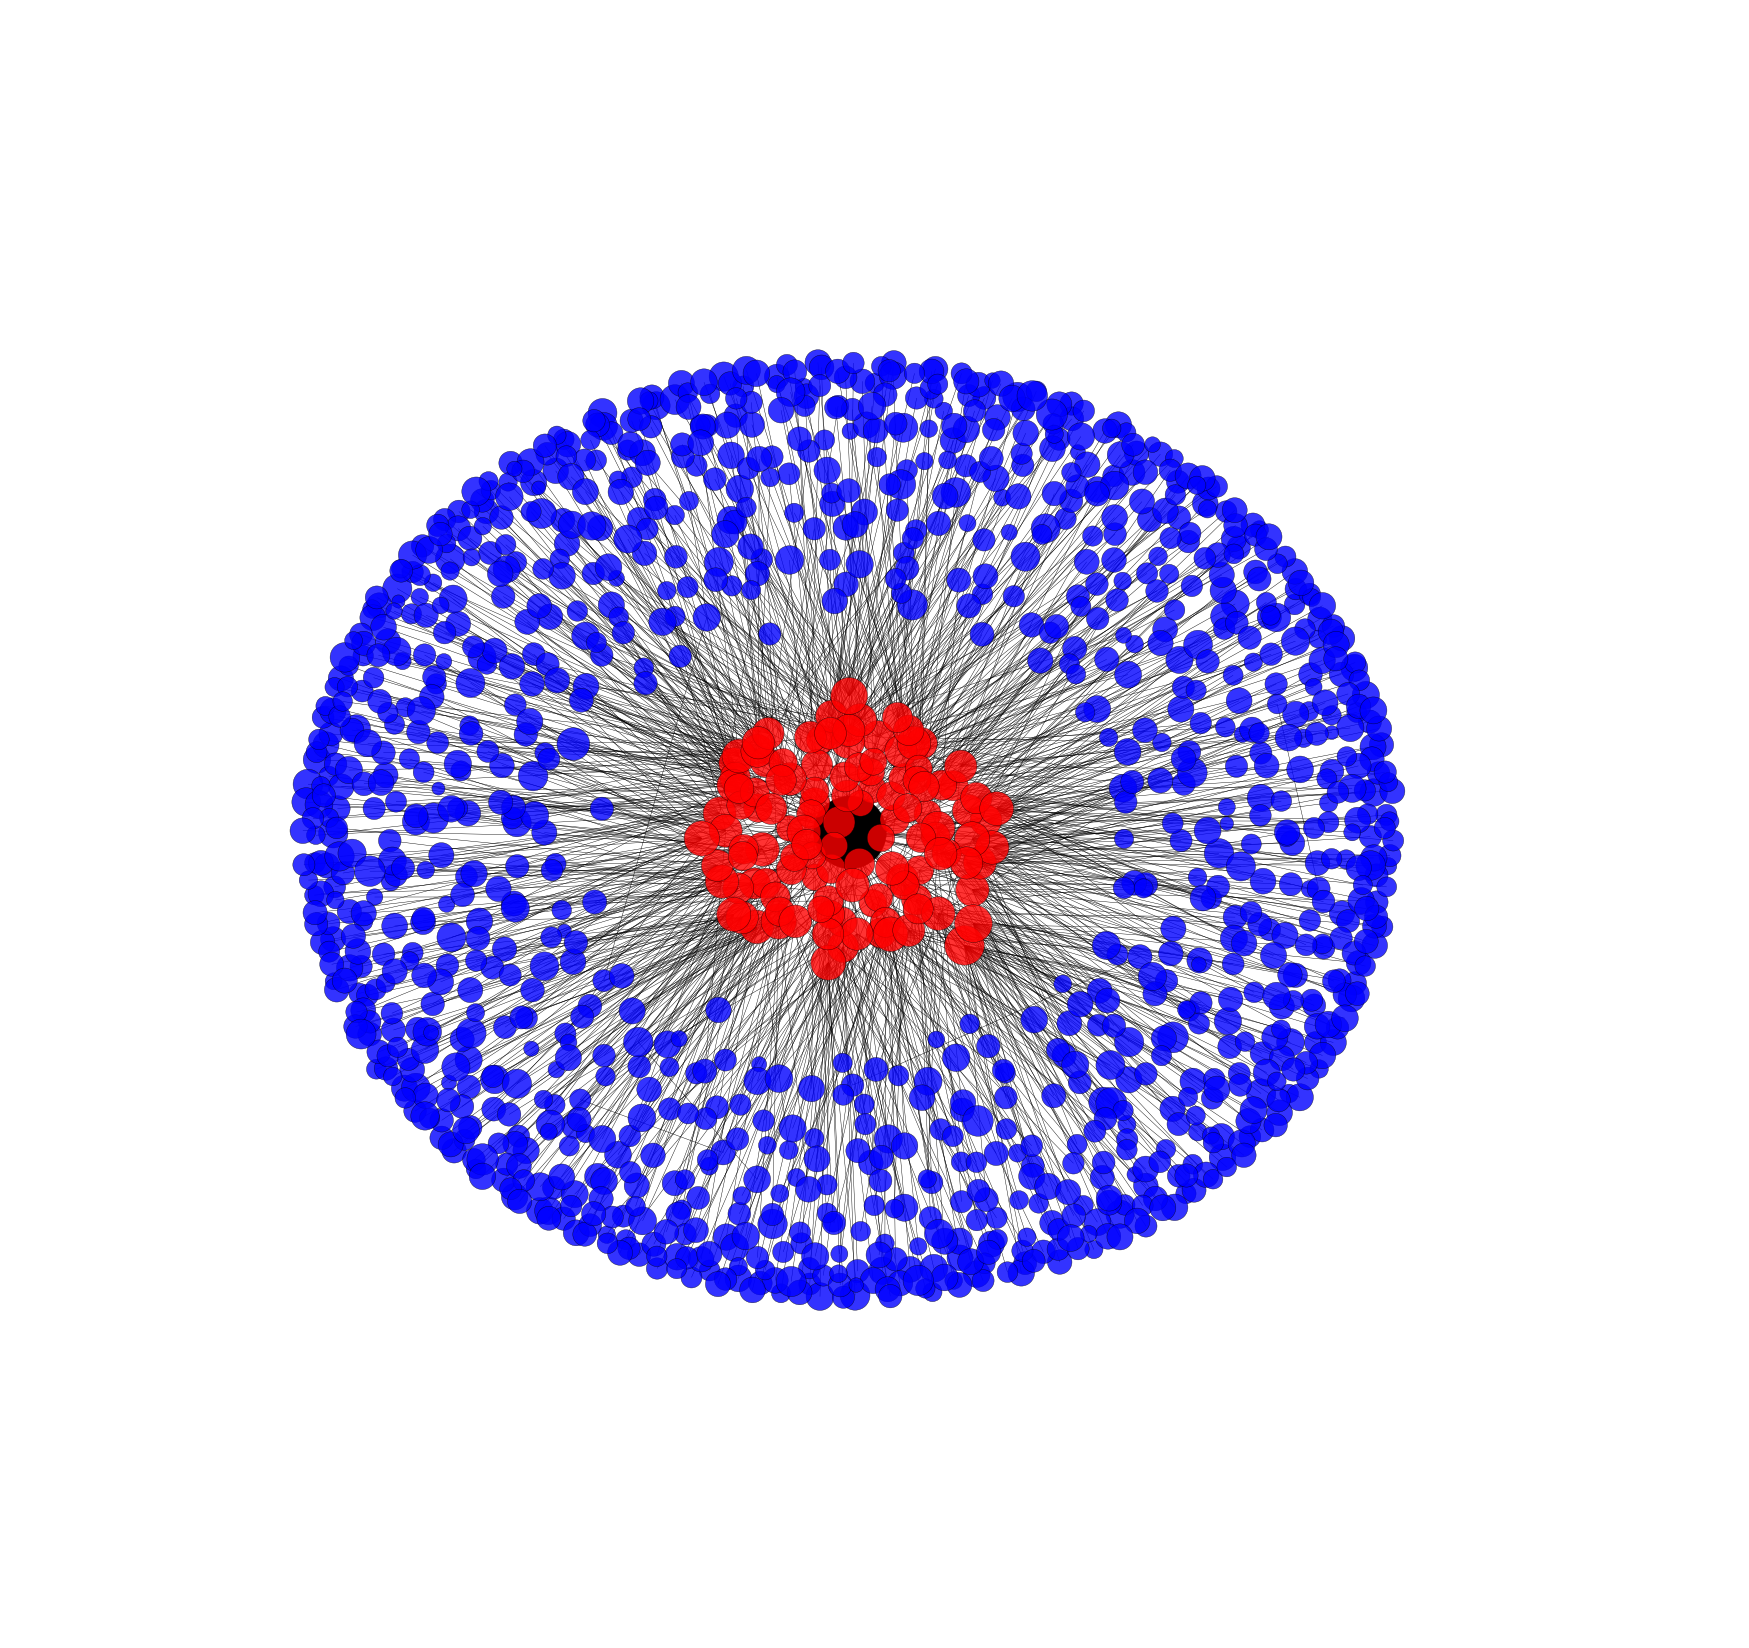
\includegraphics[width=0.49\columnwidth]{3h.png}}
\end{center}
\caption{Three snapshots of the same Poisson random graph with a growing hub at hubsizes of 20, 70, and 120. In the left column node area is proportional to eigenvector centrality, in the right column node area is proportional to non-backtracking centrality. The black node is the hub, the green (light grey) nodes are its neighbors, and all other nodes are red (grey).}
\label{fig:transition}
\end{figure}


\begin{figure}
\begin{center}
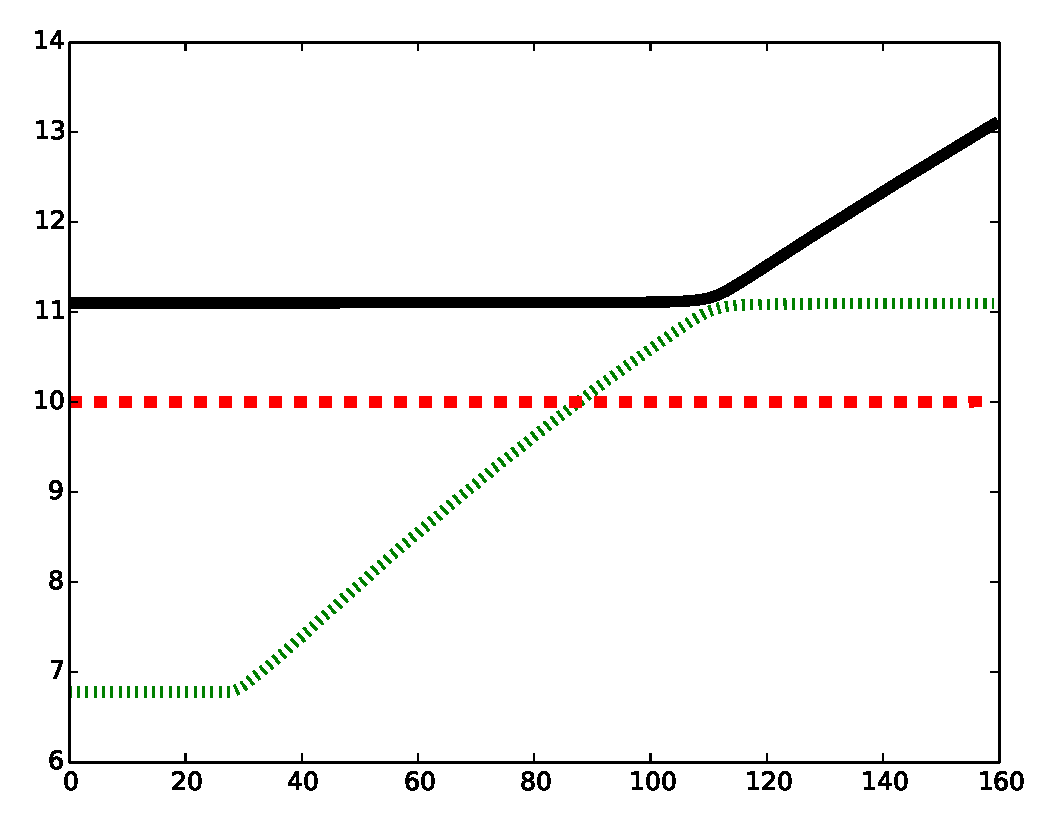
\includegraphics[width=\columnwidth]{eig.eps}
\end{center}
\caption{Eigenvalues for Poisson random graph ($n=1000000$, $c=10$) with a planted hub, as a function of hub size. The leading and second leading eigenvalues of the adjacency matrix are given by the solid \colora and dotted \colorc lines, respectively. The leading eigenvalue of the non-backtracking matrix is given by the dashed \colorb line. The same graph was used for all measurements, with hub size increments of 1.}
\label{fig:evalues}
\end{figure}
Nadakuditi and Newman give careful analysis of the spectrum of random graphs with arbitrary expected degree, and show that high degree hubs in a network generate their own eigenvalues~\cite{nadakuditi13}. For the Poisson random graph with a planted hub, they calculate a hub eigenvalue of $k_n / \sqrt{k_n - c}$ in addition to the well known eigenvalue corresponding to the average degree of $c+1$. Setting these equal to each other and solving for $k_n$, we see that the hub eigenvalue overtakes the average degree eigenvalue at
\begin{equation}
k_n = c(c+1).
\label{eqn:crossover}
\end{equation}
Figure~\ref{fig:evalues} shows the results of numerical calculations of the largest (\colora solid line) and second largest (green dashed line) eigenvalues for a Poisson random graph with a single additional hub of expected degree $k_n$, as a function of $k_n$. These values closely follow the predicted results, and we can see them crossover at $k_n = 110$, according to Eq.~\ref{eqn:crossover}. Below $k_n = 30$ we see that the hub eigenvalue has fallen into the well studied continuous band of eigenvalues, detailed by Nadakuditi and Newman~\cite{nadakuditi13}. Figure~\ref{fig:order-parameter} shows that this crossover results in a phase-transition in the eigenvector elements and localization around the hub. We measure the degree of localization of the leading eigenvector $\vec{x}$ using the order parameter $q(\vec{x})$, where $q(\vec{x}) = 1$ corresponds to the most localized eigenvector (a vector with one element equal to $1$ and the rest equal to $0$) and $q(\vec{x}) = 0$ corresponds to the least localized eigenvector (an infinitely long uniform vector)
\begin{equation}
q(\vec{x}) = \sqrt[4]{\sum_{i=1}^n x_i ^ 4}.
\label{eqn:op}
\end{equation}
We expect a small and steady increase in $q$ as the hub size increases, but instead find a dramatic phase transition where the eigenvalues crossover, as the majority of the weight of the eigenvector shifts to the hub and its neighbors.

\begin{figure}
\begin{center}
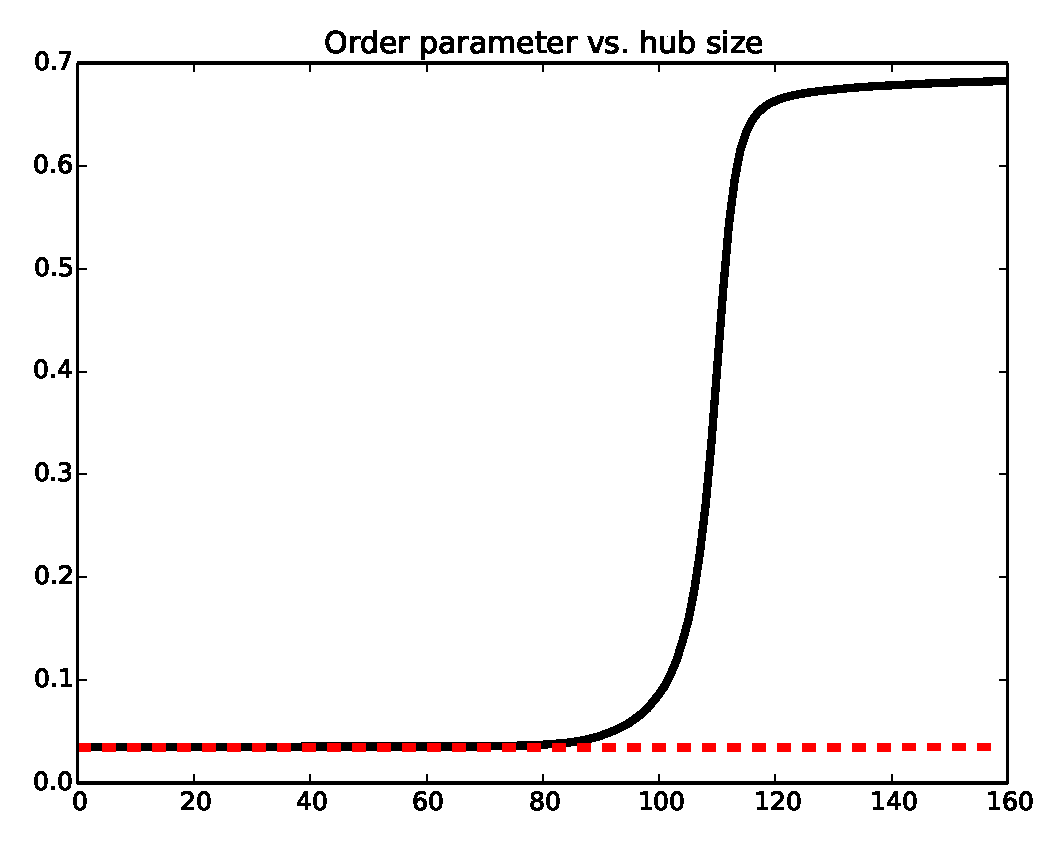
\includegraphics[width=\columnwidth]{op.eps}
\end{center}
\caption{Order parameter for Poisson random graph ($n=1000000$, $c=10$) with a planted hub, as a function of hub size. The order parameter (Eq.~\eqref{eqn:op}) of the eigenvector centrality vector is given by the solid \colora line. The order parameter of the non-backtracking centrality vector is given by the dashed \colorb line. The same graph was used for all measurements, with hub size increments of 1.}
\label{fig:order-parameter}
\end{figure}

\begin{figure}
\begin{center}
\includegraphics[width=\columnwidth]{power.eps}
\end{center}
\caption{Order parameter for a random graph ($n=1000000$) with expected degrees chosen according to a power-law distribution, as a function of power-law exponent $\beta$. The order parameter of the eigenvector centrality vector is given by the solid \colora line. The order parameter of the non-backtracking centrality vector is given by the dashed \colorb line. Order parameters were averaged over $x$ (TBD) graph instances.}
\label{fig:power-law}
\end{figure}

One might dismiss this localization, saying that the Poisson random graph is not representative of real world networks. However, eigenvector centrality may fail on any network with low average degree and high degree variability. For example, Chung~\etal\ find a similar crossover for random power-law graphs~\cite{chung03}. They show that, with high probability, networks with power-law exponent $\beta > 2.5$ have a leading eigenvalue corresponding to the square root of the maximum degree, $\sqrt{m}$, while those with $\beta < 2.5$ have a leading eigenvalue corresponding to average squared degree, $\tilde{d}$. In Figure~\ref{fig:power-law} we see this effect in action. As the power-law exponent increases the order parameter increases, despite the fact that the Gini coefficient is decreasing. % I can derive this if necessary. Currently this power-law paragraph is not as dramatic as desired, what is a good null model for how centrality should behave? Hashimoto centrality has a phase transition at 2.5, which is good?
Real world applications of eigenvector centrality to networks known to have power-law degree distributions are ubiquitous~\cite{canright06,page99}. Our results suggest that eigenvector centrality may overweight the centrality of high degree nodes~\footnote{As we show below, though network factors such as assortativity and clustering may influence the centrality measure, they do not change the presence of a high lying eigenvalues corresponding to hub nodes.}, especially when the power-law exponent is above $2.5$~\footnote{Interestingly, though many networks have a power-law exponent $2 < \beta < 2.5$, and many approach $\beta = 2.5$ we found networks with $\beta > 2.5$ to be very rare~\cite{newman03}.}.

A heuristic explanation of this failure mode follows the behavior of an echo-chamber.
A hub, having high degree, gives its neighbors high centrality. These now-important neighbors further amplify the centrality of the hub, despite the fact that their high centrality was due primarily to the high centrality of the hub.
%My idea for the following section is to show that a very localized vector gives a high eigenvalue bound. It is also very close to being an eigenvector itself (plus some constant factors), and gives an eigenvalue which is within a small factor of the (proven) leading eigenvalue. The centrality of the hub is supported by the centrality of its neighbors, whose centralities are supported by the centrality of the hub.
This can also be seen through analysis of the Rayleigh quotient, which gives a bound on the leading eigenvalue,
\begin{equation}
\lambda_1 \geq \frac{\vec{x}^{T} A \vec{x}}{\vec{x}^T\vec{x}}, \label{eq:rayleigh}
\end{equation}
for any $\vec{x}$. If we choose $\vec{x}$ to be localized around a high degree hub, $h$ of degree $k_h$:
\begin{equation*}
x_i = 
\begin{cases}
  \sqrt{k_h} & \text{if } i=h\\
  1          & \text{if } A_{ih} = 1\\
  0          & \text{otherwise}
\end{cases}.
\end{equation*}
Then
\begin{equation}
\sum_j A_{ij} x_j \geq
  \left.\begin{cases}
  k_h & \text{if } i=h\\
  \sqrt{k_h} & \text{if } A_{ih} = 1\\
  0          & \text{otherwise}
  \end{cases} \right\} = \sqrt{k_h} x_i.
  \label{eq:adj_ineq}
\end{equation}
Multiplying both sides of Eq.~\eqref{eq:adj_ineq} by $x_i$, summing over $i$, and using Eq.~\eqref{eq:rayleigh},
\begin{equation*}
\lambda_1 \geq \frac{\vec{x}^{T} A \vec{x}}{\vec{x}^T\vec{x}} \geq \sqrt{k_h}.
\end{equation*}
Though an approximation, we see that a vector localized around the hub is very nearly an eigenvector with an eigenvalue which increases as the hub size increases. The hub's large eigenvector element is supported by its neighbors' large eigenvector elements, while the neighbors' large eigenvector elements are supported by the hub's large eigenvector element.

Non-backtracking centrality avoids this problem by making a node's centrality proportional to its neighbors centralities, but \emph{excluding} the portion of each neighbor's centrality due to the node itself. We formally define non-backtracking centrality in terms of the non-backtracking matrix, defined as follows~\cite{newman13}. One first converts the network into a directed network by replacing each undirected edge $\{i, j\}$ with two directed edges pointing in opposite directions, which we label indicating the direction they point, $i \rightarrow j$ and $j \rightarrow i$. The non-backtracking matrix $\mat{B}$ is a $2m \times 2m$ non-symmetric matrix with one row and one column for each directed edge and elements
\begin{equation}
B_{i\rightarrow j, k \rightarrow l} = \delta_{il}(1-\delta_{jk}),
\end{equation}
where $\delta_{ij}$ is the Kronecker delta. In other words, all elements are zero unless edge $i\rightarrow j$ points out of the same vertex that edge $k \rightarrow l$ points into, and edges $i \rightarrow j$ and $k \rightarrow l$ are not pointing in opposite directions between the same pair of vertices. Let $\vec{v}$ be the leading eigenvector of $\mat{B}$, normalized and chosen with positive elements. We define a node $i$'s non-backtracking centrality, $b_i$, to be the sum of the elements of $v$ for $i$'s incoming edges:
\begin{equation*}
b_i = \sum_{j\rightarrow i} v_{j\rightarrow i}
\end{equation*}

We can similarly define an edge matrix version of the Adjacency matrix, $\mat{A'}$:
\begin{equation*}
A'_{i\rightarrow j, k \rightarrow l} = \delta_{il}
\end{equation*}
Letting $\vec{v}$ be the leading eigenvector of $\mat{A'}$, node $i$'s eigenvector centrality $a_i$ can be expressed
\begin{equation}
a_i = \sum_{j\rightarrow i} v_{j\rightarrow i}.
\end{equation}
Thus these two centrality measures differ only by their inclusion or exclusion of non-backtracking edges, which, in the limit of dense graphs, are a vanishing fraction of the edges in each row. Thus these centrality measures are only noticeably different for sparse graphs.

Non-backtracking centrality neatly resolves the failure cases of eigenvector centrality discussed above. In the right column of Figure~\ref{fig:transition}, which displays nodes proportional to their centrality for three increasing hub sizes, we see that non-backtracking centralities increase gradually, in contrast to the results of the left column for identical graphs. Additionally, before the transition in the third row, node eigenvector and non-backtracking centralities are roughly equal. In Figure~\ref{fig:evalues}, the \colorb dashed line displays the leading eigenvalue of $\mat{B}$ as a function of hub size. We notice there is no eigenvalue transition, instead the eigenvalue stays constant at the average degree of $c$ (not $c+1$ because backtracking edges are excluded), which is hardly effected by hub growth in a million node network.

The \colorb dashed line in Figure~\ref{fig:order-parameter} demonstrates the order parameter for the non-backtracking centrality vector, $q(\vec{b})$ as a function of hub size. Instead of a localization transition as before, we see negligible changes as hub size increases. Our results for power-law graphs are most interesting. The \colorb dashed line in Figure~\ref{fig:power-law} shows $q(\vec{b})$ for a random graph with a power-law degree distribution as a function of the power-law exponent $\beta$. We find opposite behavior from the power-law case, decreasing $q$ for increasing $\beta$. Table~\ref{tab:power} helps to explain this by showing centralities for two graphs with different power-law parameters. A graph with low power-law parameter gives more high degree nodes, and thus is less likely to give one anomalously high-degree hub. The node of degree 5461, for $\beta = 2.9$ has significantly higher degree than the rest of its neighbors, leading to extreme localization in the eigenvector centrality vector. Non-backtracking centrality avoids this localization and distributes more centrality to the plethora of low-degree nodes, leading to a lower $q$.

Naive computation of non-backtracking centrality from the $2m \times 2m$ non-backtracking matrix can be significantly more laborious than the computation of eigenvector centrality from the $n \times n$ adjacency matrix. From the non-backtracking matrix Krzakala~\etal\ derive a $2n \times 2n$ matrix, 
\begin{equation}
\left(
 \begin{array}{c|c}
 0 & \mat{I} \\
  \hline
  \mat{I} - \mat{D} & \mat{A}
 \end{array} \right),
\end{equation}
where $\mat{I}$ is the identity matrix and $\mat{D}$ as the matrix with node degrees along its diagonal, for which the bottom half of the leading eigenvector is equal to $\vec{b}$, the non-backtracking centrality vector. This matrix only has $2n$ more non-zero entries than the original adjacency matrix, and gives a much more efficient method of computing non-backtracking centrality.

\begin{table}
\centering
\begin{tabular}{|c|c|c|} \hline
\multicolumn{3}{|c|}{$\beta=2.1$} \\ \hline
Degree & Eigenvector & Non-backtracking \\ \hline
42172 & 0.140 & 0.129 \\ \hline
67039 & 0.186 & 0.155 \\ \hline
92258 & 0.229 & 0.171 \\ \hline
92563 & 0.230 & 0.171 \\ \hline \hline
\multicolumn{3}{|c|}{$\beta=2.9$} \\ \hline 
Degree & Eigenvector & Non-backtracking \\ \hline
923  & 0.014 & 0.045 \\ \hline
1513 & 0.018 & 0.069 \\ \hline
1867 & 0.022 & 0.085 \\ \hline
5461 & 0.710 & 0.171 \\ \hline
\end{tabular}
\caption{Centralities for the highest degree nodes from two random graphs of size $n=1000000$, with power-law distributed expected degrees but two different power-law exponents.}
\label{tab:power}
\end{table}

We've shown that non-backtracking serves as a principled fix to some shortcomings of eigenvector centrality, while remaining equivalent in the limit of dense graphs. However, non-backtracking centrality is not without it's own faults. Perhaps its most serious shortcoming is its behavior on graphs without cycles, or trees. Consider the computation of non-backtracking centrality, starting from the leaves and progressing towards the root of the tree. Each leaf's centrality is simply proportional to the centrality of its one neighbor, and thus our non-backtracking requirement prevents any leaf from contributing to the centrality of its neighbor. By the same reasoning, no node which is distance 1 from the leaves can contribute to the centrality of its one neighbor which is distance 2 from the leaves. Following this reasoning, we find that no nodes are able to contribute to the centrality of any other, and the tree represents a degenerate case with all eigenvalues equal to 0. This is clearly undesirable, as many other centralities are, and should be, well defined on tree graphs. Improving non-backtracking centrality for tree graphs remains a promising area for future research.
% leave the relation of belief propagation and core-periphery structure for another paper


\bibliography{travis}

\end{document}
